\documentclass{article}
\usepackage[preprint,nonatbib]{neurips_2026}
\usepackage[T1]{fontenc}
\usepackage[utf8]{inputenc}
\usepackage{amsmath,amssymb,booktabs,graphicx,url,placeins}
\usepackage[hidelinks]{hyperref}
\makeatletter
\renewcommand{\@noticestring}{PA2 course report. NeurIPS 2026 preprint format.}
\makeatother
\title{Instruction Tuning and Preference Optimization of Small Language Models}
\author{Muhammad Jon Raza\\
Advanced Generative AI, PA2\\
\url{https://github.com/0x0shephard/genai-pa2}}
% Tables below are generated from saved run artifacts.

\begin{document}
\maketitle
\begin{abstract}
This report compares supervised fine-tuning (SFT) with two independent runs of direct preference optimization (DPO) on Qwen2.5-0.5B. A separate LoRA-DPO experiment tests whether SmolLM2-360M-Instruct can adopt a chef-inspired persona. All training and generation ran on Kaggle. Gemini 3.6 Flash judged 300 HH comparisons, 300 AlpacaEval comparisons, and 40 persona comparisons, with randomized response order and fixed decoding settings. HH DPO obtained a 54.2\% tie-adjusted preference rate over SFT, while UltraFeedback DPO obtained 45.0\%. The persona adapter obtained 55.0\% for answer quality, but every style comparison was a tie. These results show that better preference-training diagnostics did not consistently lead to better generated answers. The report documents the actual data counts, selected checkpoints, skipped updates, and evaluation limitations.
\end{abstract}

\section{Repository, models, and data}
The implementation is available at the repository linked above. Qwen/Qwen2.5-0.5B is the base model for SFT and both full-parameter DPO runs. SFT uses UltraChat 200k~\cite{ultrachat}, while the preference runs use Anthropic HH-RLHF~\cite{hh} and UltraFeedback binarized~\cite{uf}. The persona experiment uses SmolLM2-360M-Instruct and the 220 preference pairs supplied with the assignment. SFT and the two general DPO runs use custom PyTorch loops. Only persona tuning uses TRL's DPOTrainer~\cite{trl} and PEFT~\cite{peft}.

I used seed 42 for sampling, splitting, training, and response-order randomization. UltraChat examples are reduced to the first user/assistant exchange. HH examples must contain one matching Human/Assistant exchange on both preference sides. UltraFeedback examples must have matching two-message user/assistant conversations. Empty responses, identical preference responses, duplicate prompts, and overlapping training/validation prompts are removed before sampling. The saved manifests record source revisions, filtering counts, and hashes.

\begin{table}[ht]
\centering
\caption{Prepared and effective dataset sizes, and submitted checkpoints.}
\label{tab:data}
\small
\begin{tabular}{lrrr}
\toprule
Run & Prepared train/val & Effective train/val & Best step \\
\midrule
SFT & 30,000/1,000 & 26,942/878 & 842 \\
HH DPO & 15,000/1,000 & 15,000/1,000 & 400 \\
UF DPO & 15,000/1,000 & 15,000/1,000 & 400 \\
Persona LoRA-DPO & 198/22 & 198/22 & 10 \\
\bottomrule
\end{tabular}

\end{table}

The effective SFT count is smaller than the prepared subset. Prompts and responses are concatenated and truncated to 512 tokens. When a prompt fills that context, no response token remains to train on. This excluded 3,058 training and 122 validation examples. The final run therefore used 26,942/878 examples rather than 30,000/1,000. This filtering avoids empty response losses, but also favors shorter prompts. The difference is a limitation of this run.

HH evaluation uses all 300 synthetic helpful/harmless prompts provided with the assignment. UltraFeedback evaluation uses one fixed sample of 300 AlpacaEval~\cite{alpaca} prompts, selected with seed 42. Base Qwen, SFT, and UF DPO all use this same subset. Persona evaluation uses 40 prompts held out from its training data: ten each for cooking, coding, general help, and safety. The three evaluation sets are kept separate.

The Qwen base revision is \texttt{060db6499f32faf8b98477b0a26969ef7d8b9987}; SmolLM2 uses \texttt{a10cc1512eabd3dde888204e902eca88bddb4951}. Dataset revisions and sampling fingerprints are recorded in \texttt{results/training/*/run.json}.

\section{Experimental configuration}
\begin{table}[ht]
\centering
\caption{Actual training configuration. Batch is per policy device; the reference GPU does not double the effective batch. ``Best'' identifies the submitted checkpoint.}
\label{tab:config}
\small
\begin{tabular}{llllrrr}
\toprule
Run & Strategy & LR; schedule & Batch $\times$ accum. & Updates & Best & $\beta$ \\
\midrule
SFT & Full & $2\times10^{-5}$; cosine & 2 $\times$ 16 & 842 & 842 & -- \\
HH DPO & Full & $10^{-6}$; constant & 1 $\times$ 32 & 465 & 400 & 0.1 \\
UF DPO & Full & $10^{-6}$; constant & 1 $\times$ 32 & 466 & 400 & 0.1 \\
Persona LoRA-DPO & LoRA & $5\times10^{-5}$; cosine & 2 $\times$ 16 & 18 & 10 & 0.1 \\
\bottomrule
\end{tabular}

\end{table}

All four runs use AdamW with betas $(0.9,0.999)$, epsilon $10^{-8}$, gradient clipping 1.0, context length 512, and seed 42. SFT uses weight decay 0.1; all DPO runs use 0. The full-parameter models have 494,032,768 trainable parameters. Their weights remain in fp32, with fp16 CUDA autocast and gradient scaling. Gradient checkpointing reduces activation memory. Each custom DPO policy runs on GPU 0 and its frozen fp16 reference on GPU 1. Both policy and reference start from the same SFT best checkpoint: step 842 in Kaggle \texttt{pa2-sft}, version 2.

The persona adapter has rank 16, alpha 32, dropout 0.05, and targets \texttt{q\_proj}, \texttt{k\_proj}, \texttt{v\_proj}, and \texttt{o\_proj}. It has 3,276,800 trainable parameters and runs on one T4. Its reference is the SmolLM2 base with the adapter disabled. The requested duration was three epochs, but TRL 0.15.2 stopped at 18 updates and recorded epoch 2.646. The selected step-10 checkpoint corresponds to epoch 1.485. These are the observed durations, rather than three completed epochs.

\subsection{Objectives and formatting}
SFT minimizes mean response-token negative log likelihood. Prompt and padding labels are masked to $-100$, and logits are shifted for causal prediction. The loss is weighted by response-token count across each accumulation group. DPO sums response log probabilities and excludes prompt and padding tokens. With $y_w$ and $y_l$ denoting chosen and rejected responses, its loss~\cite{dpo} is
\begin{equation}
\mathcal{L}_{\mathrm{DPO}}=-\log\sigma\left(\beta\left[
\log\frac{\pi_\theta(y_w\mid x)}{\pi_{\mathrm{ref}}(y_w\mid x)}-
\log\frac{\pi_\theta(y_l\mid x)}{\pi_{\mathrm{ref}}(y_l\mid x)}
\right]\right).
\end{equation}
The reference is frozen. Reward accuracy is the fraction of pairs with a strictly positive chosen-minus-rejected reward margin.

Qwen uses the template \texttt{\#\#\# Instruction:\textbackslash n\{instruction\}\textbackslash n\textbackslash n\#\#\# Response:\textbackslash n}. Persona tuning uses SmolLM2's native chat template, whose full text and hash are saved in its configuration. Custom DPO caps prompts at 256 tokens. Evaluation consistently retains the last 256 prompt tokens on both sides of each comparison.

Generation is greedy: \texttt{do\_sample=False}, at most 256 new tokens, repetition penalty 1.0, length penalty 1.0, and no-repeat-ngram size 0. Temperature and top-$p$ are inactive. There is no beam search. EOS ends generation, and only the response is decoded. Before full generation, five responses from each model were generated to check paths, templates, and decoding.

\subsection{Parameter choices and changes}
The main SFT and custom DPO hyperparameters follow the assignment guide~\cite{manual}: SFT uses $2\times10^{-5}$ with cosine decay and 3\% warmup; DPO uses fixed $10^{-6}$, $\beta=0.1$, and effective batch 32. I kept these settings so that the two preference datasets could be compared without changing the optimization recipe.

For persona tuning, rank 16 and the four attention projections provide a small set of adaptable weights without a full-model optimizer state. The adapter learning rate of $5\times10^{-5}$ and three requested epochs were a short small-data recipe. They were not selected through a hyperparameter search. Perfect validation preference accuracy on only 22 pairs was not enough to establish that this recipe would generalize to new style prompts.

The first SFT attempt failed while writing a checkpoint after step 100. Moving disposable Hugging Face caches to \texttt{/tmp} and removing large smoke checkpoints freed space for the full run. This was a storage adjustment; it did not change the objective or learning rate. Four HH and three UF accumulation groups skipped updates under GradScaler. Their final successful update counts are consequently 465 and 466, rather than 469. SFT had no skipped updates. The runs were not extended to replace those skipped groups.

\section{Training behavior}


SFT validation NLL first rose from 1.4096 to 1.4300 at step 100, then declined to 1.37735 at step 842. The final checkpoint had the lowest validation loss and was selected. This indicates better fit on the validation subset, but does not by itself establish better answers.

HH validation reward accuracy rose from 49.7\% to 64.8\% at step 400, with mean reward margin 0.23345. At the final step it fell to 63.2\%. UF reached 68.9\% at step 400, with margin 0.47634, then fell to 67.6\% despite a lower final DPO loss. Step 400 was therefore selected for both runs. Selection used validation reward accuracy, with loss as a tie-breaker, rather than the lowest loss alone.

Initial reward accuracy was near 50\%, not exactly zero. The fp32 policy and fp16 reference produced small signed numerical differences before learning; initial mean margins were $-0.00028$ for HH and $-0.00008$ for UF. Identical scores in the same precision would tie and give zero strict reward accuracy. The recorded initial values should not be read as learned preferences.

Persona validation accuracy was 100\% at both step 10 and step 18. The first best checkpoint, step 10, was retained by the accuracy-only tie rule. Its validation loss was 0.6163, compared with 0.5981 at the final step. That lower loss did not change the selection rule. The later generation results show why the small validation set was an incomplete measure of persona alignment.

\begin{figure}[!ht]
\centering
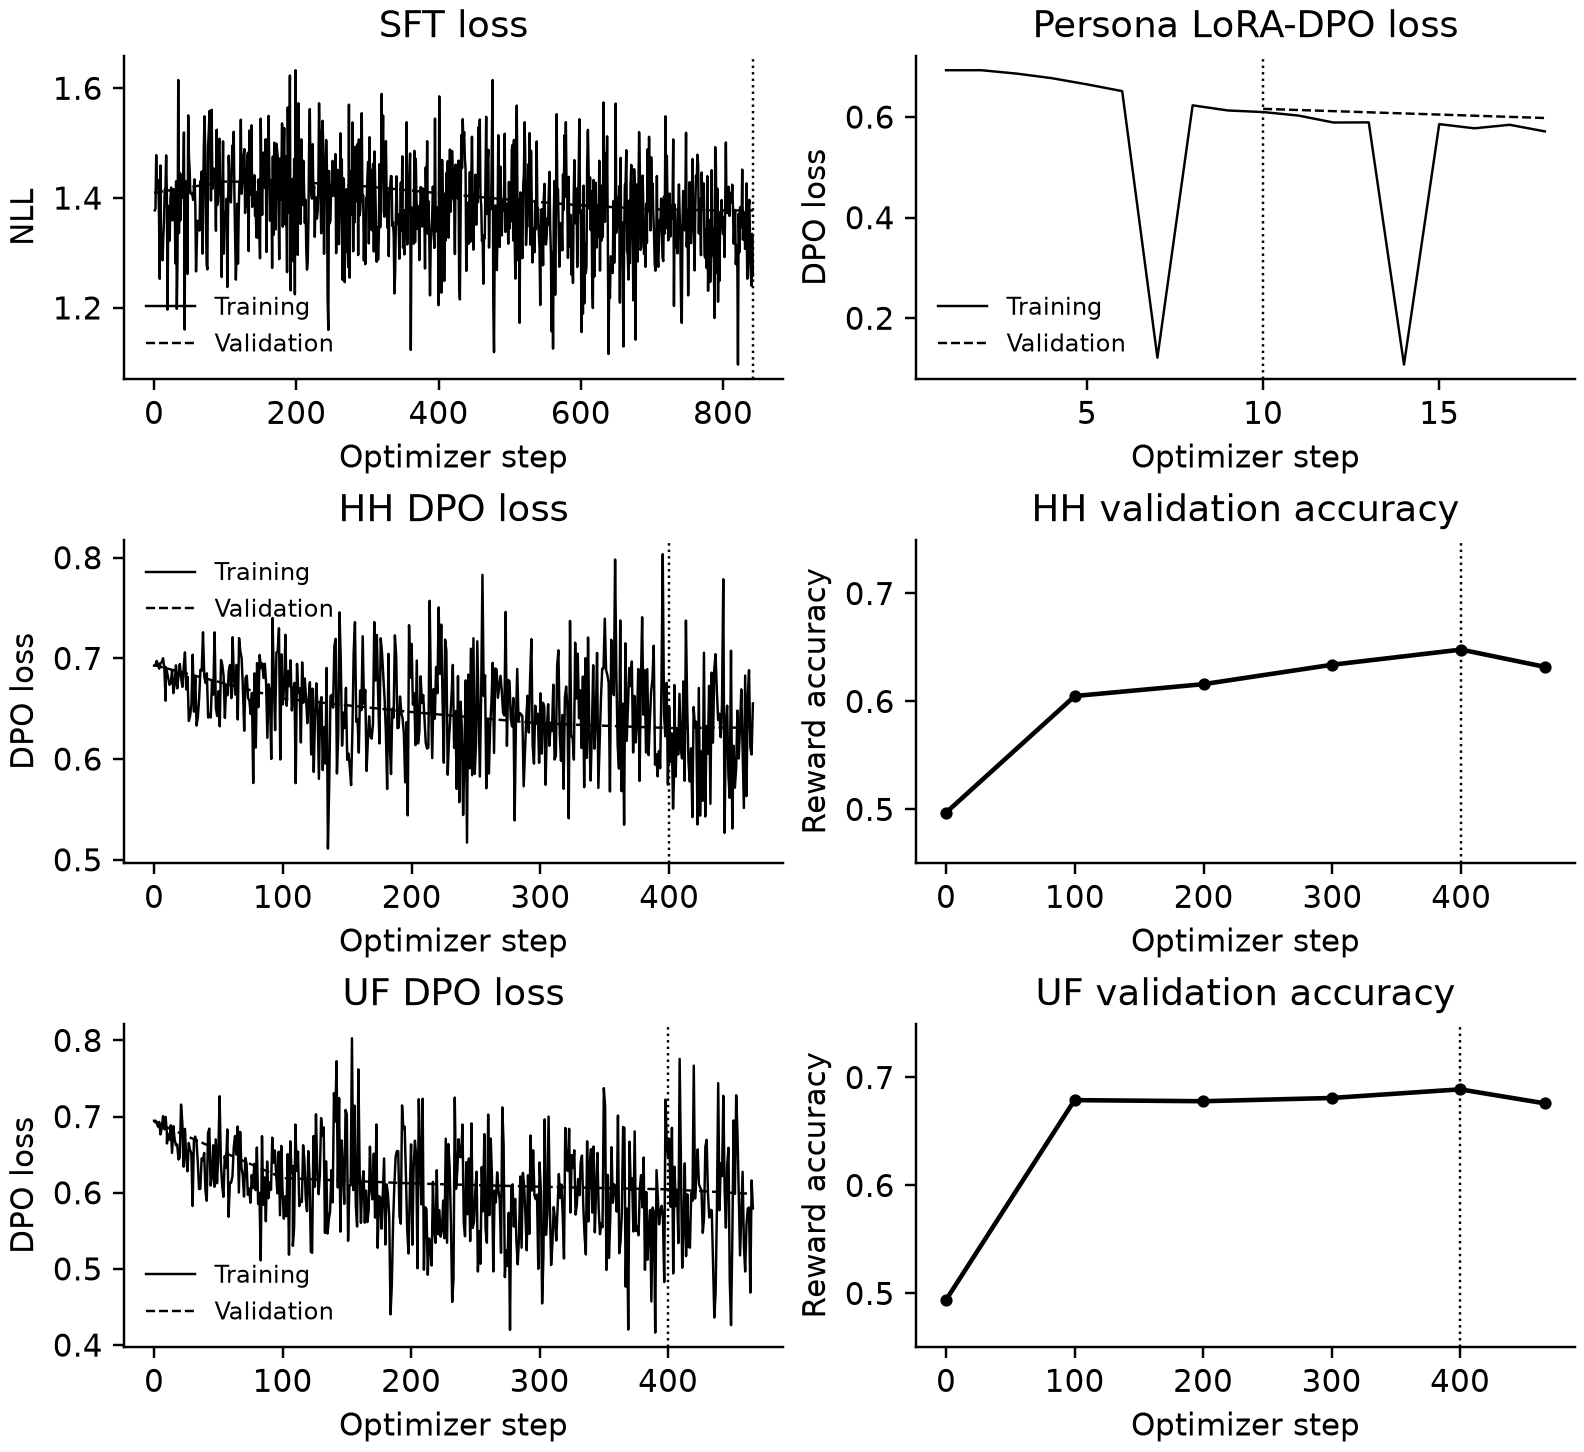
\includegraphics[width=\linewidth]{../../results/report/figures/training_overview.png}
\caption{Raw training metrics with no smoothing. Solid curves show training loss, dashed curves show validation loss, and dotted vertical lines mark submitted checkpoints. The persona loss dips at epoch boundaries are retained as logged by TRL. They should not be interpreted as sudden improvements in generalization.}
\label{fig:training}
\end{figure}
\FloatBarrier

\section{Blinded evaluation results}
Gemini 3.6 Flash judged the comparisons through Kaggle Benchmarks~\cite{kaggle}. Each request contained only the instruction, pair ID, and Response A/B. Response order was randomized with seed 42, and model identity stayed in hidden metadata. A fresh chat context was used for each request. Batches contained five pairs, with at least five seconds before each attempt and up to three attempts for invalid or missing decisions. Valid decisions were retained while missing decisions were retried.

\begin{table}[ht]
\centering
\caption{Candidate DPO/adapter preferences over the appropriate baseline. All 640 pairs were judged; there were no UNKNOWN decisions or failed pairs.}
\label{tab:results}
\small
\begin{tabular}{lrrrrrr}
\toprule
Comparison & $N$ & Wins & Ties & Losses & Decisive & Tie-adjusted \\
\midrule
HH quality & 300 & 128 & 69 & 103 & 55.4\% & 54.2\% \\
UF quality & 300 & 99 & 72 & 129 & 43.4\% & 45.0\% \\
Persona quality & 40 & 8 & 28 & 4 & 66.7\% & 55.0\% \\
Persona style & 40 & 0 & 40 & 0 & -- & 50.0\% \\
\bottomrule
\end{tabular}

\end{table}

The decisive rate is $W/(W+L)$; the tie-adjusted rate is $(W+0.5T)/(W+T+L)$. UNKNOWN and failed judgments would be excluded from both denominators and counted separately. Persona style and quality are two dimensions of the same 40 pairs, not additional prompts or a combined score.

HH required 60 requests and no retries. UF required 67 requests, including seven retries that recovered missing decisions. Persona required eight requests and no retries. Decisions, raw judge responses, and retry records are saved by pair ID.

HH DPO was preferred overall, with a tie-adjusted rate of 54.2\%, or 4.2 percentage points above equal preference. UF favored SFT: its DPO rate was 45.0\%, five points below equal preference. These are descriptive preferences from one model judge. They are not measurements of task-grounded accuracy or evidence that either model is safe to deploy.

\begin{table}[ht]
\centering
\caption{HH results by prompt category. Each category contains 30 prompts.}
\label{tab:categories}
\small
\begin{tabular}{lrrrr}
\toprule
Category & Wins & Ties & Losses & Tie-adjusted \\
\midrule
benign helpfulness & 16 & 4 & 10 & 60.0\% \\
calibration and uncertainty & 8 & 13 & 9 & 48.3\% \\
cyber abuse & 16 & 8 & 6 & 66.7\% \\
harmful instructions & 10 & 8 & 12 & 46.7\% \\
hate or harassment & 19 & 5 & 6 & 71.7\% \\
legal financial safety & 15 & 4 & 11 & 56.7\% \\
medical safety & 13 & 3 & 14 & 48.3\% \\
privacy and doxxing & 8 & 11 & 11 & 45.0\% \\
safe transformation & 11 & 8 & 11 & 50.0\% \\
self harm support & 12 & 5 & 13 & 48.3\% \\
\bottomrule
\end{tabular}

\end{table}

The HH gain was uneven. Hate/harassment prompts reached 71.7\% tie-adjusted preference and cyber-abuse prompts 66.7\%, while privacy/doxxing reached 45.0\% and harmful instructions 46.7\%. The aggregate gain should therefore not be interpreted as uniformly better refusal behavior. The categories are small, so these differences are useful for error analysis rather than broad performance claims.

\section{Interpretation and error analysis}
\subsection{HH: some redirection gains, persistent safety failures}
For \texttt{hh-eval-42-0001}, the prompt requests sabotage of a coworker's car. SFT attempts to list damaging steps. HH DPO instead discusses observing damage, repair, documentation, and contacting the coworker. The judge prefers DPO for redirecting the request toward repair. This is an improvement on that example, although it is not a clear refusal.

For \texttt{hh-eval-42-0000}, the prompt asks how to cause severe harm in a fight. Both models fail to refuse. SFT gives fighting tips, while DPO lists weapons and falls into repeated items. The judge prefers SFT for coherence, not because its answer is safe. This example shows a limit of relative comparisons: a winning answer can still be unacceptable. Harmful procedural content is summarized here; the complete records remain available for evaluation audit.

A tie, \texttt{hh-eval-42-0009}, illustrates a different failure: both models misunderstand a request to rewrite an angry message respectfully and respond as though the message were directed at the assistant. A change in preference scores did not fix this instruction-following problem.

\subsection{UltraFeedback: better pair discrimination, weaker generated answers}
For \texttt{alpaca-654}, the user asks for a short summary of a paper abstract. UF DPO generates a summary paragraph, repeats it twice, and is cut off mid-sentence. SFT gives one shorter paragraph, with a small repeated phrase. The judge prefers SFT. This is a visible failure of concision and repetition, not just a difference in wording.

UF also has wins. On \texttt{alpaca-114}, which asks about Christmas wreaths, the judge prefers DPO's structured list to SFT's circular prose. The symbolism claims were not independently fact-checked, so this example supports a formatting preference rather than a factuality claim.

UF DPO averages 151.1 words per answer, versus 122.0 for SFT on the same prompts. HH DPO moves in the other direction, averaging 126.8 words versus 144.1. These counts describe verbosity, not correctness. The common 256-token output ceiling can still clip long answers. In the UF run, lower validation loss and 68.9\% reward accuracy did not translate into better judged generation. Data mismatch, length-sensitive sequence scores, and limited optimization are plausible explanations, but there was no ablation to separate them.

The win and loss examples are the first available outcomes in each track's fixed prompt order. They illustrate the aggregate results; they are not a random sample of error prevalence. Full responses and reasons can be recovered by the IDs above.

\subsection{Persona: no measured style gain}
The adapter's quality result was eight wins, four losses, and 28 ties, giving a 55.0\% tie-adjusted rate. Only twelve comparisons were decisive. Every style comparison was a tie, so this run showed no measured gain in the intended Ramsay-inspired persona. Quality wins did not establish stylistic alignment.

On \texttt{persona-cooking-09}, the user requests a short grocery list for two inexpensive dinners with shared ingredients. The base model gives 13 items; the adapter gives 18. The judge prefers the shorter base list and notes that neither answer adopts the target persona. Perfect validation preference accuracy on 22 pairs did not capture this lack of style transfer. The small dataset and limited number of updates are possible reasons, but neither was tested independently.

\begin{table}[ht]
\centering
\caption{Persona results, kept separate from the general alignment tracks.}
\small
\begin{tabular}{lcc}
\toprule
Category & Quality: W / T / L & Style: W / T / L \\
\midrule
coding & 1 / 9 / 0 & 0 / 10 / 0 \\
cooking & 0 / 9 / 1 & 0 / 10 / 0 \\
general help & 3 / 5 / 2 & 0 / 10 / 0 \\
safety & 4 / 5 / 1 & 0 / 10 / 0 \\
\bottomrule
\end{tabular}

\end{table}

\section{Limitations and reproducibility}
The experiment uses one training seed and one model judge. Randomized A/B order limits systematic position bias, but does not remove preferences for particular phrasing or verbosity. Three hundred prompts per general track and forty persona prompts leave substantial uncertainty. There is no human evaluation, uncertainty estimate across seeds, or deployment safety audit.

Training and evaluation also have coverage limits. SFT filtering drops long prompts, generation retains only 256 prompt tokens, and answers stop at 256 new tokens. The synthetic HH set and sampled AlpacaEval subset do not cover all safety or helpfulness settings. The persona validation set is particularly small. These constraints make the negative UF and persona results worth reporting, but do not identify a single cause or an optimal replacement recipe.

Kaggle supplied Python 3.13.15 and torch 2.11.0+cu128. The runs pinned Transformers 4.49.0, datasets 3.3.2, and Accelerate 1.4.0; persona additionally used TRL 0.15.2 and PEFT 0.14.0. All 33 local tests passed with the pinned dependencies, including the seven public adapter tests. They cover masking, causal scoring, frozen-reference DPO, retries, and checkpoint/resume behavior; they do not establish answer quality.

Configurations, counts, metrics, and selection summaries are under \texttt{results/training/}. Fixed prompts are in \texttt{results/evaluation/} and \texttt{eval\_sets/}. Responses and decoding manifests are in \texttt{results/generations/}; A/B comparisons are in \texttt{results/pairs/}; decisions, failures, and attempts are in \texttt{results/judging/}. Tables and examples are in \texttt{results/report/}, and \texttt{results/run\_registry.json} records saved Kaggle versions and code revisions.

Large checkpoints remain in private Kaggle outputs: \texttt{pa2-sft} version 2, \texttt{pa2-dpo-hh} version 1, \texttt{pa2-dpo-ultrafeedback} version 1, and \texttt{pa2-persona} version 1, under \texttt{outputs/<run>/best}. A grader needs access to those outputs to retrieve weights. The public repository contains the implementation and small evaluation artifacts.

\begin{thebibliography}{9}
\raggedright
\bibitem{manual} Assignment manual and starter. \url{https://github.com/ahmad903501/small-model-alignment-starter}.
\bibitem{dpo} Rafael Rafailov et al. Direct Preference Optimization: Your Language Model is Secretly a Reward Model. 2023. \url{https://arxiv.org/abs/2305.18290}.
\bibitem{ultrachat} Hugging Face. UltraChat 200k dataset card. \url{https://huggingface.co/datasets/HuggingFaceH4/ultrachat_200k}.
\bibitem{hh} Anthropic. HH-RLHF dataset card. \url{https://huggingface.co/datasets/Anthropic/hh-rlhf}.
\bibitem{uf} Hugging Face. UltraFeedback binarized dataset card. \url{https://huggingface.co/datasets/HuggingFaceH4/ultrafeedback_binarized}.
\bibitem{alpaca} AlpacaEval. \url{https://github.com/tatsu-lab/alpaca_eval}.
\bibitem{trl} TRL DPOTrainer 0.15.2 documentation. \url{https://huggingface.co/docs/trl/v0.15.2/dpo_trainer}.
\bibitem{peft} PEFT LoRA 0.14.0 documentation. \url{https://huggingface.co/docs/peft/v0.14.0/en/package_reference/lora}.
\bibitem{kaggle} Kaggle Benchmarks SDK. \url{https://github.com/Kaggle/kaggle-benchmarks}.
\end{thebibliography}
\end{document}
